\documentclass{article}

\usepackage{kern}

\begin{document}


    \begin{figure}
        \centering
        \begin{subfigure}[t]{0.45\textwidth}
            \centering
            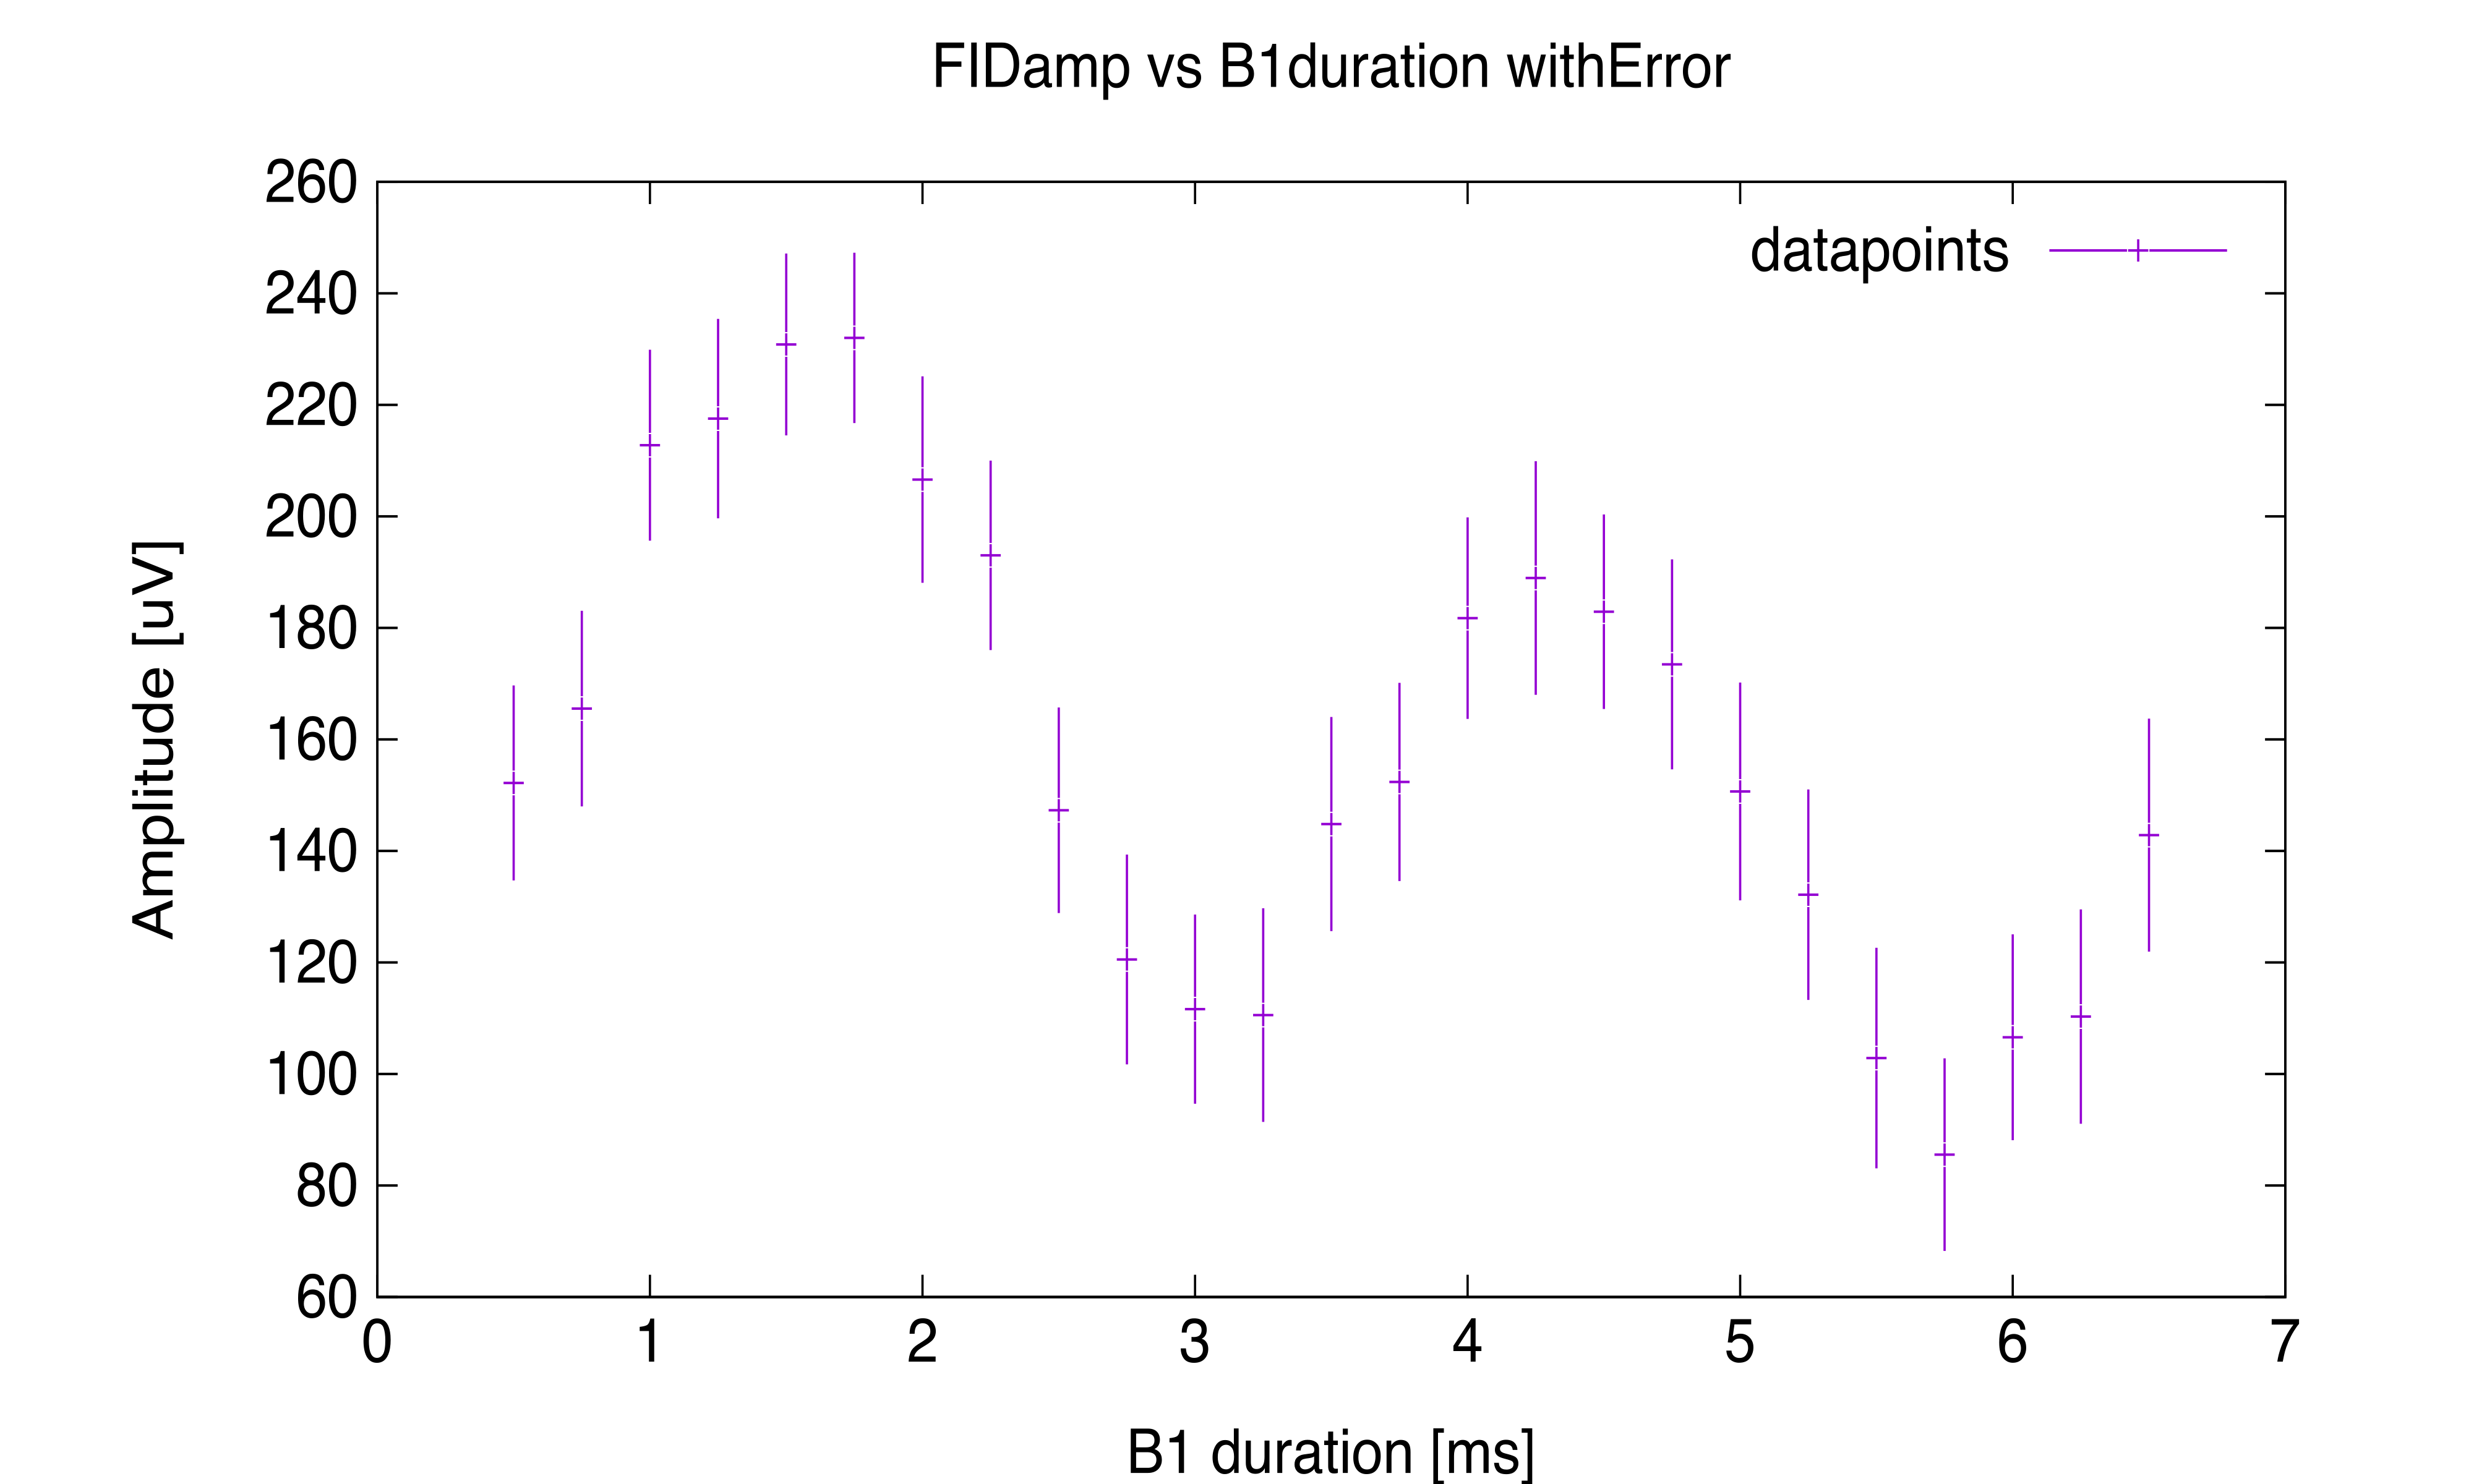
\includegraphics[width=6cm]{../Bilddateien/B1DurationFast_FIDamp_vs_B1duration_withError.png}
            \caption{Messung der FID-Amplitude mit Fehlerbalken in Abhängigkeit der B1-Dauer.}
            \label{fig:5:FastFIDampVsB1durationWithError}
        \end{subfigure}
        \
        \begin{subfigure}[t]{0.45\textwidth}
            \centering
            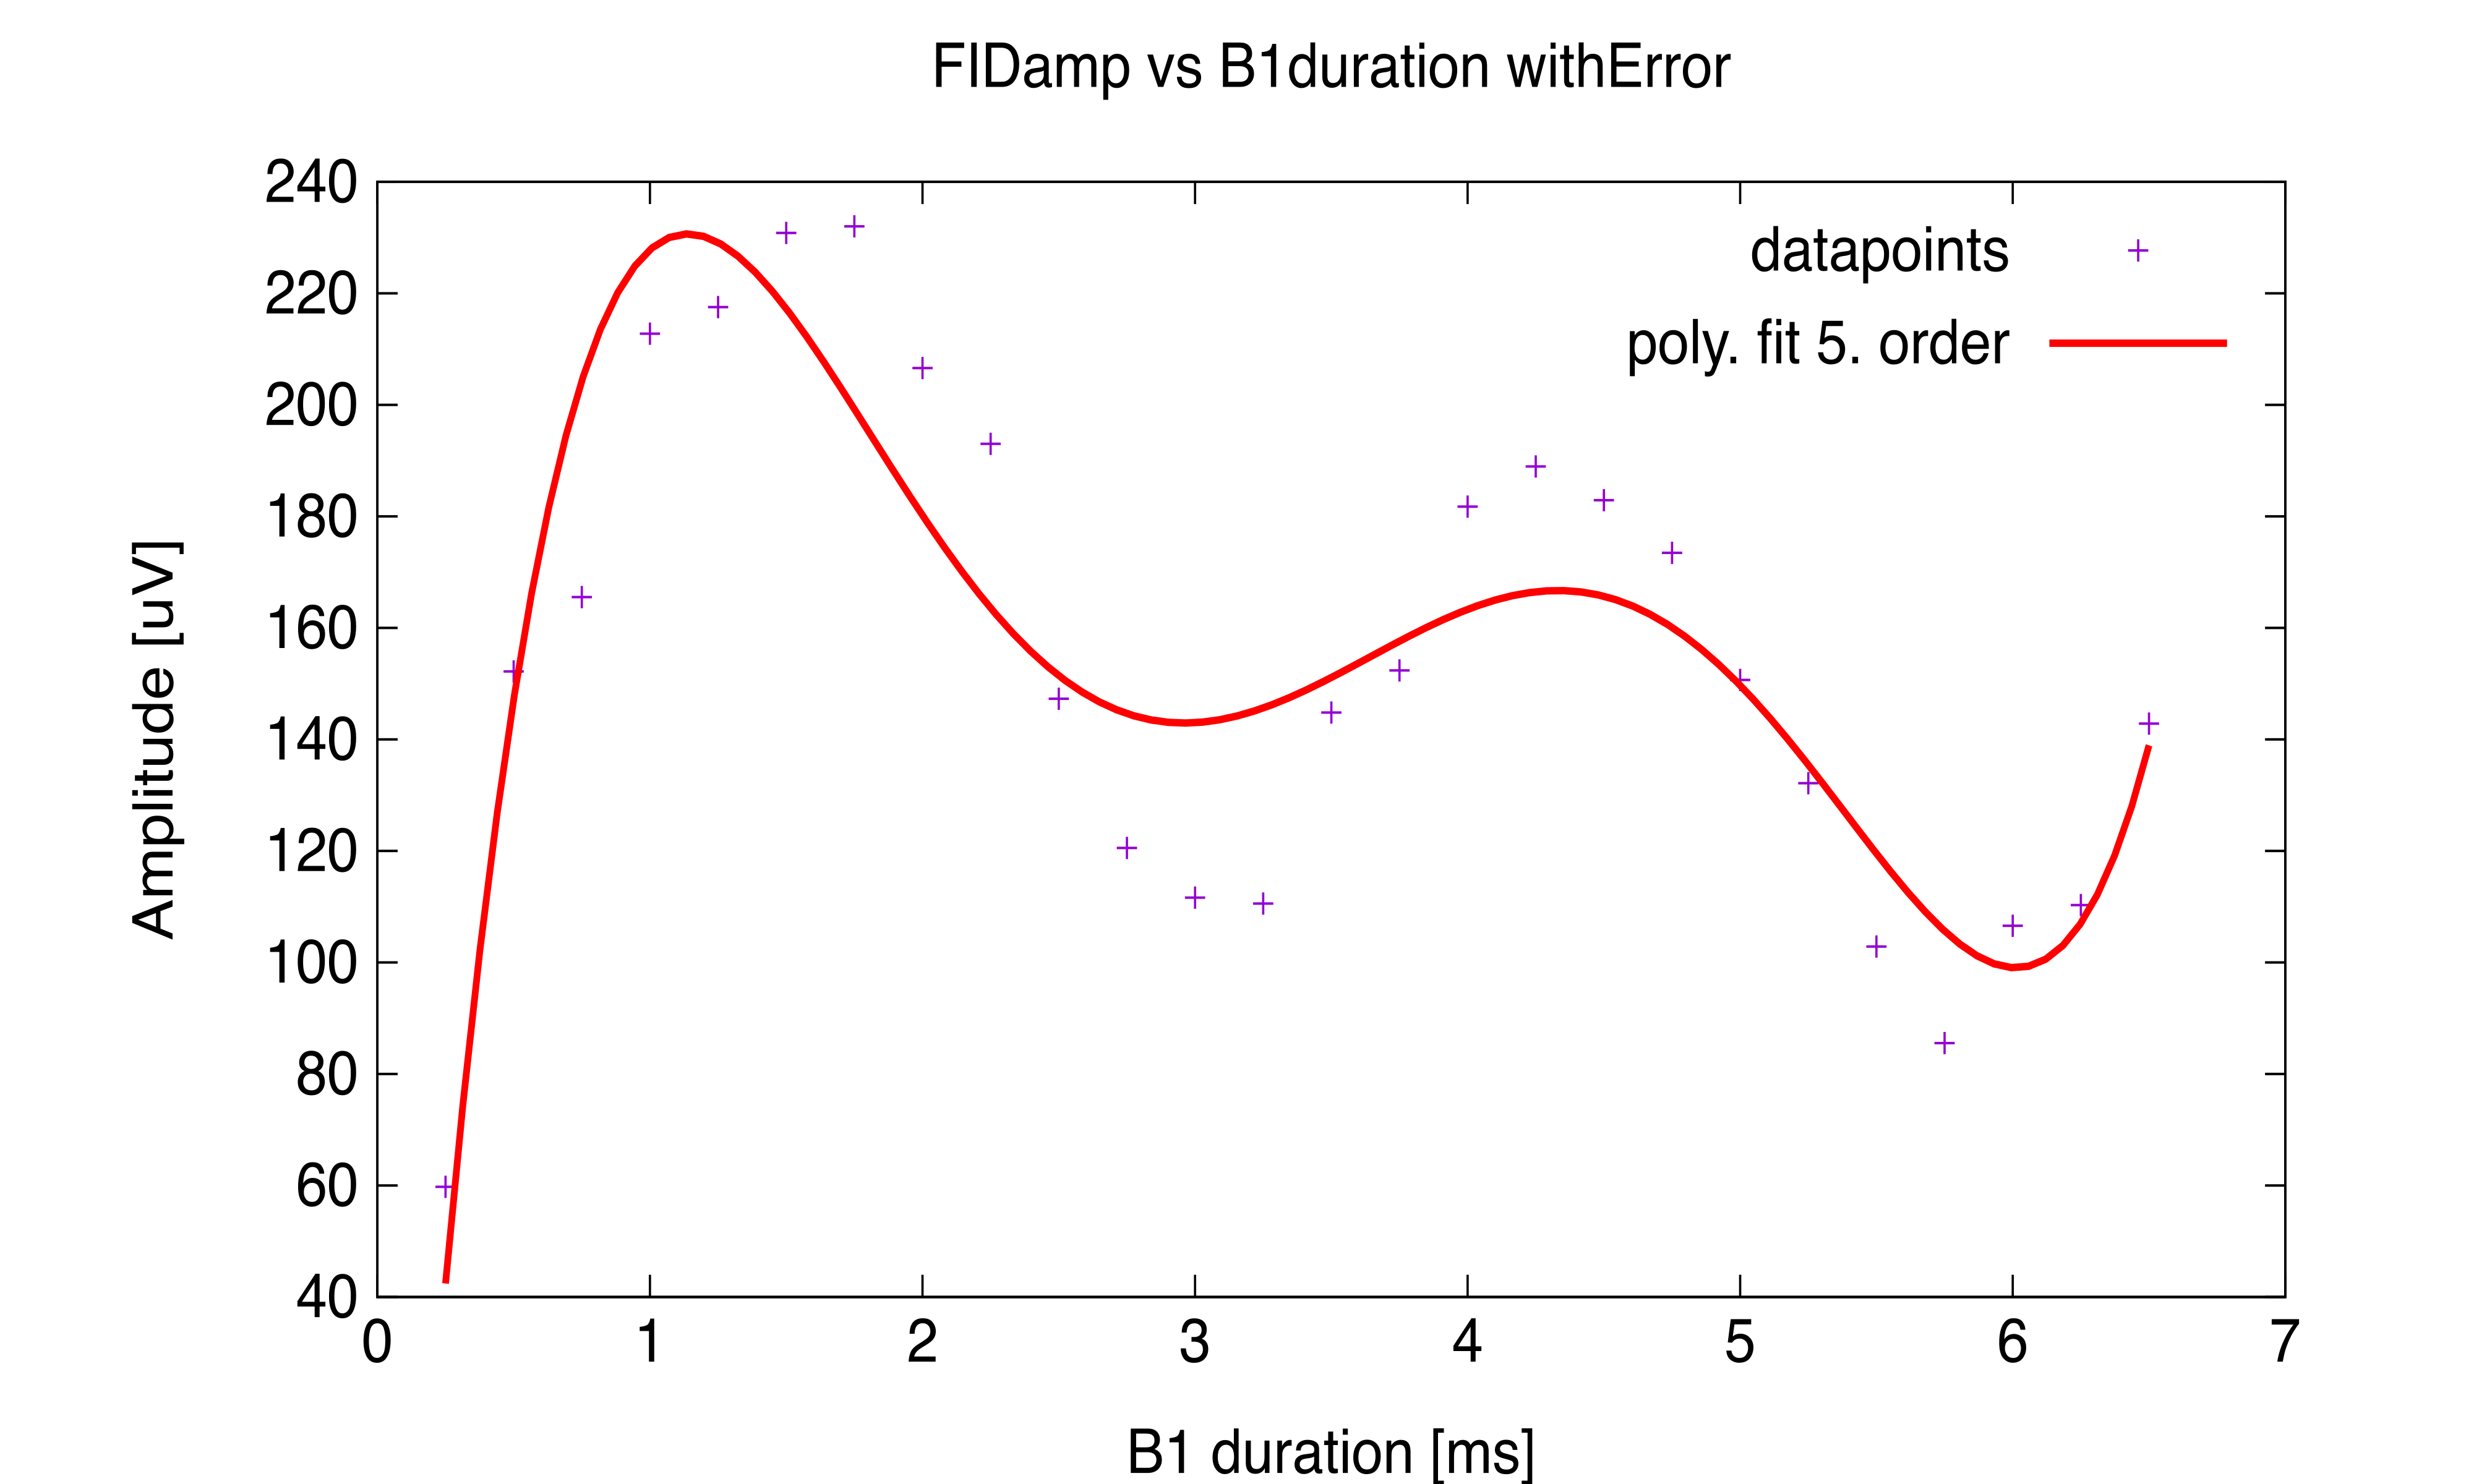
\includegraphics[width=6cm]{../Bilddateien/B1DurationFast_FIDamp_vs_B1duration_withError_poly.png}
            \caption{Messung der FID-Amplitude in Abhängigkeit der B1-Dauer mit polynomialer Kurvenanpassung fünfter Ordnung.}
            \label{fig:5:FastFIDampVsB1duration}
        \end{subfigure}
        \caption{Messung der FID-Amplitude in Abhängigkeit der B1-Dauer.}
    \end{figure}
\end{document}